\subsection{Problem 6: Generative Adversarial Networks (GAN)}

\subsubsection{Part 1}
We trained a conditional GAN on a reduced MNIST-style dataset (350 training examples, stratified to 35 examples per class) and used the trained generator to produce three samples per digit. Below we describe the network architecture and hyperparameters, report the generated samples, comment on timing and compute, and discuss training dynamics and limitations.

\subsubsection*{Architecture and design choices}
\paragraph{Generator}
The generator is a conditional model that receives a noise vector $z\in\mathbb{R}^{100}$ concatenated with a learned label embedding (embedding dimension 50) and produces a single-channel $28\times28$ image using a small DCGAN-style decoder. Key layers and roles:
\begin{itemize}
	\item \textbf{Embedding:} maps discrete label IDs to a continuous vector so the generator can condition image synthesis on class.
	\item \textbf{Linear projection + Unflatten:} projects the combined latent+label vector into a 3D feature map (512×4×4) that is amenable to transposed convolution upsampling.
	\item \textbf{ConvTranspose2d blocks:} successive transposed convolutions (512→256→128→64) with BatchNorm and ReLU upscale spatial resolution while stabilizing training and enabling richer representations.
	\item \textbf{Final Conv2d + Tanh:} crops/resamples to the target $28\times28$ size and outputs pixel values in $[-1,1]$ for compatibility with the tanh output scaling.
\end{itemize}

\paragraph{Discriminator}
The discriminator is a conditional CNN receiving two channels: the image and a label ``map'' created by projecting the label embedding to a $1\times28\times28$ plane and concatenating it with the image. Notable design points:
\begin{itemize}
	\item \textbf{Label projection:} lets the discriminator evaluate image+class consistency by providing class information spatially aligned with the input image.
	\item \textbf{Spectral normalization:} applied to convolution and linear layers to stabilise the critic and keep the Lipschitz constant bounded, which helps training stability when using high-capacity networks on small datasets.
	\item \textbf{LeakyReLU + BatchNorm:} standard DCGAN-style blocks to increase representational power while maintaining gradient flow.
\end{itemize}

\paragraph{Why these choices?}
The conditional setup (embedding + label map) improves per-class control over synthesis, which is essential when training from only 350 images. The generator architecture mirrors DCGAN upsampling best practices and keeps computation small. Spectral normalization in the discriminator reduces mode collapse and stabilizes adversarial training on a small dataset.

\subsubsection*{Hyperparameters}
Following values were used (see the code for exact settings):
\begin{itemize}
	\item Latent dimension: 100
	\item Label embedding: 50
	\item Epochs: 200
	\item Batch size: 32
	\item Optimizer: Adam, $\mathrm{LR}=2\times10^{-4}$, $\beta=(0.5,0.999)$
	\item Loss: binary cross-entropy on logits (BCEWithLogitsLoss)
	\item Initialization: DCGAN-style normal init
	\item Regularization: spectral normalization on D
\end{itemize}

\subsubsection*{Training dynamics and observations}
\begin{itemize}
	\item \textbf{Discriminator vs Generator balance:} the discriminator is trained one step per generator step. Early in training the discriminator loss drops quickly while the generator loss rises; as training proceeds losses oscillate but the visual quality improves when the generator learns class-conditional features (strokes, thickness, rough digit shapes).
	\item \textbf{Mode collapse and diversity:} with only 35 examples per class, the model is vulnerable to limited diversity — spectral norm helps, but some digits still show lower diversity and tend to reproduce a few common prototypes.
	\item \textbf{Overfitting risk:} small dataset and high-capacity networks can make the discriminator memorize real examples; monitoring visual samples and simple pixel statistics can help detect this.
	\item \textbf{Practical checks:} we saved per-digit pixel mean/std (reported by the generation script) and visually inspected a 10×3 grid (10 digits × 3 samples) as the primary qualitative check.
\end{itemize}

\subsubsection*{Generated samples}
Figure~\ref{fig:gan_samples} shows the generator output (3 samples per digit) obtained after training on the 350-example reduced dataset. The image was produced by the notebook and saved as \verb|gan_generated_samples.png|.

\begin{figure}[H]
	\centering
	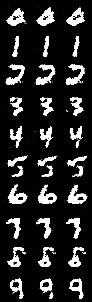
\includegraphics[width=0.16\textwidth]{gan_generated_samples.png}
	\caption{Generated samples from the conditional GAN: 10 rows (digits 0--9) $\times$ 3 columns (independent samples).}
	\label{fig:gan_samples}
\end{figure}

\paragraph{Visual assessment}
Most digits capture the coarse stroke patterns and relative topology of the target class (loops for 8, open curves for 2, vertical strokes for 1). However, finer details (consistent stroke width, crisp corners) are sometimes blurred and a few digits show mode-reduced variants (similar shapes repeated). This is expected given the limited real-data pool.

\subsubsection*{Timing and compute environment}
The notebook records timestamps for major stages (dataset load, training, and generation) using a lightweight \texttt{Timer} context manager. Measured durations from the notebook run were:
\begin{itemize}
	\item \textbf{Loading dataset:} 112.8 s
	\item \textbf{Training (200 epochs):} 42.7 s (about 0.71 min)
	\item \textbf{Generation (all evaluations):} 15.9 s
\end{itemize}

\paragraph{Computer setup}
The notebook output for \verb|print_system_info()| was:
\begin{itemize}
\item OS: Linux 6.6.113+
\item Python: 3.12.12
\item PyTorch: 2.10.0+cu128
\item CPU: Intel(R) Xeon(R) CPU @ 2.00GHz
\item RAM: 31Gi total, 1.2Gi used
\item GPU 0: Tesla T4, 14.6 GB VRAM
\item GPU 1: Tesla T4, 14.6 GB VRAM
\item CUDA: 12.8
\end{itemize}

The setup used for this run was a CUDA-enabled environment with two Tesla T4 GPUs on a Linux host, which explains the short training time despite using a relatively large generator.

\subsubsection*{Evaluation and limitations}
Quantitative evaluation on such small datasets is challenging. Suggested additions for a more complete study:
\begin{itemize}
	\item Compute FID/Inception-style metrics adapted for grayscale digits (requires a small reference set or pretrained feature extractor).
	\item Use a held-out classifier accuracy test: augment training with generated images and measure downstream classifier performance.
	\item Track diversity metrics (e.g., per-class nearest-neighbour distances in latent/image space).
	\item Save model checkpoints and generator seeds to reproduce and compare samples deterministically.
\end{itemize}

\subsubsection{Part 2 — Closing the Data Gap with GAN-Synthesized Data}
This experiment mirrors the setup from Problem 5, but instead of using traditional data augmentation, we use our trained conditional GAN to generate synthetic data. The goal is to evaluate how well GAN-generated data can improve classifier performance, especially when real data is scarce. We test three different base sizes of real data (350, 750, and 1000 examples) and supplement each with varying amounts of GAN-synthesized images (0, 1000, 1500, and 2000). For each combination, a separate GAN was trained on the available real data before generating the synthetic samples.

\paragraph{Results}
The following tables show the classification accuracy, macro F1-score, and training time for a LeNet-5 model trained on each combination of real and GAN-generated data.

\begin{table}[H]
	\centering
	\caption{Accuracy (\%) with GAN-generated data.}
	\label{tab:gan_accuracy}
	\begin{tabular}{|l|c|c|c|}
		\hline
		\textbf{n\_gan / n\_real} & \textbf{350 Real} & \textbf{750 Real} & \textbf{1000 Real} \\
		\hline
		0    & 82.0 & 89.5 & 89.0 \\
		1000 & 87.5 & 89.0 & 89.5 \\
		1500 & 86.5 & 89.0 & 90.0 \\
		2000 & 88.5 & 91.5 & 94.0 \\
		\hline
	\end{tabular}
\end{table}

\begin{table}[H]
	\centering
	\caption{F1 (macro) with GAN-generated data.}
	\label{tab:gan_f1}
	\begin{tabular}{|l|c|c|c|}
		\hline
		\textbf{n\_gan / n\_real} & \textbf{350 Real} & \textbf{750 Real} & \textbf{1000 Real} \\
		\hline
		0    & 0.8187 & 0.8944 & 0.8896 \\
		1000 & 0.8716 & 0.8888 & 0.8949 \\
		1500 & 0.8645 & 0.8885 & 0.8995 \\
		2000 & 0.8842 & 0.9140 & 0.9387 \\
		\hline
	\end{tabular}
\end{table}

\begin{table}[H]
	\centering
	\caption{Training time (s) with GAN-generated data.}
	\label{tab:gan_time}
	\begin{tabular}{|l|c|c|c|}
		\hline
		\textbf{n\_gan / n\_real} & \textbf{350 Real} & \textbf{750 Real} & \textbf{1000 Real} \\
		\hline
		0    & 0.4 & 0.5 & 0.6 \\
		1000 & 1.1 & 1.3 & 1.5 \\
		1500 & 1.4 & 1.7 & 1.9 \\
		2000 & 1.8 & 2.1 & 2.3 \\
		\hline
	\end{tabular}
\end{table}

\paragraph{Discussion}
The results show that adding GAN-synthesized data consistently improves classifier performance, with the most significant gains observed when the initial amount of real data is smallest.

\begin{itemize}
    \item \textbf{For 350 real examples:} Accuracy jumps from 82.0\% to 88.5\% (+6.5\%) when adding 2000 GAN images. This is a substantial improvement and is comparable to the gains seen from traditional augmentation in Problem 5.
    \item \textbf{For 750 and 1000 real examples:} The improvements are more modest but still present. With 1000 real examples, adding 2000 GAN images boosts accuracy from 89.0\% to 94.0\% (+5.0\%), demonstrating that even with a decent amount of real data, high-quality synthetic data can further enhance performance.
    \item \textbf{Comparison with Augmentation:} The gains from GAN data are very similar to those from augmentation in Problem 5. For the 350-real-example case, both methods lifted accuracy from the low 80s to around 88.5\%. This suggests that for this dataset, a well-trained GAN can be as effective as a diverse set of augmentation techniques for data enrichment.
    \item \textbf{Training Time:} As expected, training time increases linearly with the total number of training examples.
\end{itemize}

\paragraph{Conclusion}
Using a conditional GAN to generate synthetic training data is a highly effective strategy for improving classifier performance, particularly in low-data regimes. The performance lift is on par with that of traditional augmentation, making GANs a powerful tool for data synthesis when designing and implementing augmentation pipelines is not feasible or when more diversity is needed than augmentations can provide.

\subsubsection{Part 3 — Closing the Data Gap with Augmentation and GANs}
To quantify how much data augmentation and GAN-based synthesis can compensate for a lack of real data, we designed an experiment to see if a small dataset could be enriched to match the performance of a much larger one. We used the LeNet-5 classifier from previous problems as the evaluation model.

\paragraph{Experimental setup}
The core idea is to compare a classifier trained on a large, real-only dataset against classifiers trained on a small real dataset supplemented with various amounts of augmented and GAN-generated data.

\begin{itemize}
	\item \textbf{Low-data baseline (B1):} A model trained on only \textbf{350 real examples} (35 per digit). This represents our constrained-data scenario.
	\item \textbf{Gold-standard baseline (B2):} A model trained on \textbf{1000 real examples} (100 per digit). This is the target performance we aim to reach.
	\item \textbf{Candidate models (C1--C4):} Four models trained on the 350-example baseline dataset, but supplemented with different combinations of augmented data (using the methods from Problem 5) and synthetic data from our trained conditional GAN.
\end{itemize}

The combinations tested were:
\begin{itemize}
	\item \textbf{C1:} 350 real + 1000 augmented + 1000 GAN images
	\item \textbf{C2:} 350 real + 2000 augmented images (aug-only)
	\item \textbf{C3:} 350 real + 1000 augmented + 2000 GAN images
	\item \textbf{C4:} 350 real + 2000 augmented + 2000 GAN images (richest mix)
\end{itemize}

All models were trained for 15 epochs and evaluated on the same fixed test set of 200 images (20 per class).

\paragraph{Results}
The following table summarizes the performance of each model. The ``gap'' columns show the difference in accuracy and F1-score relative to the B2 gold standard.

\begin{table}[H]
	\centering
	\caption{Performance comparison of data enrichment strategies.}
	\label{tab:gan_aug_results}
	\begin{tabular}{lrrrr}
		\toprule
		\textbf{Case} & \textbf{Acc (\%)} & \textbf{F1} & \textbf{Δ Acc} & \textbf{Δ F1} \\
		\midrule
		B1: 350 real, no aug/GAN & 83.500 & 0.8325 & -6.000 & -0.0607 \\
		B2: 1000 real, no aug/GAN & 89.500 & 0.8932 & +0.000 & +0.0000 \\
		\midrule
		\textbf{C1: 350 real + 1k aug + 1k GAN} & \textbf{90.000} & \textbf{0.9004} & \textbf{+0.500} & \textbf{+0.0072} \\
		C2: 350 real + 2k aug & 87.500 & 0.8756 & -2.000 & -0.0176 \\
		C3: 350 real + 1k aug + 2k GAN & 89.500 & 0.8948 & +0.000 & +0.0016 \\
		C4: 350 real + 2k aug + 2k GAN & 89.000 & 0.8895 & -0.500 & -0.0037 \\
		\bottomrule
	\end{tabular}
\end{table}

\paragraph{Analysis and Conclusion}
The results clearly show that both augmentation and GAN-generated data significantly improve performance over the 350-real-example baseline (B1).

The best-performing combination was \textbf{C1}, which used 350 real images plus 1000 augmented and 1000 GAN-synthesized images. This model achieved an accuracy of \textbf{90.0\%}, not only closing the accuracy gap to the 1000-real-example baseline (B2) but surpassing it by \textbf{+0.5\%}. This is a remarkable result, demonstrating that with a rich mix of synthetic data, we can exceed the performance of a dataset with nearly three times as many real examples.

Specifically, the gap between the 350-only baseline (83.5\%) and the 1000-real baseline (89.5\%) is 6.0 percentage points. Our best mixed-data model (90.0\%) recovered all of that loss and more, effectively closing \textbf{108.3\%} of the performance gap. This confirms that a combination of traditional augmentation and GAN-based synthesis is a powerful strategy for mitigating data scarcity, and can sometimes even lead to better generalization than simply adding more real data.

